\chapter{Popis řešení}

V~této kapitole rozebereme obecné vlastnosti našeho řešení. Nejprve detailněji popíšeme použitý algoritmus a~opodstatníme některá koncepční rozhodnutí, která jsme učinili jako důsledek použitého frameworku. Poté nastíníme obecný způsob fungování programu a~zamyslíme se nad rozdíly mezi různými variantami řešeného problému.

\section{DPLL($T$) s~vyčerpávající propagací teorie}\label{dpllt}

Připomeňme si metodu \icode{SetTrue} uvedenou v~sekci \ref{smt}. Ta slouží k~přidání nového omezení do kontextu řešiče teorie. Řešič může volitelně jako návratovou hodnotu uvést nějakou množinu literálů, které detekoval jako důsledky vzniklé přidáním právě tohoto omezení. Může přitom hlásit např. jen \uv{zjevné} důsledky, popřípadě nemusí vracet vůbec žádné. Pokud jsme je ale schopni nacházet v~rozumém čase, nahlášené důsledky jsou užitečnou informací pro hlavní engine, poněvadž pro něj mohou výrazně zmenšit velikost rozhodovacího stromu.

Varianta DPLL($T$) s~vyčerpávající propagací teorie přidává pro \icode{SetTrue} silnou podmínku; řešič musí vrátit \emph{všechny} literály ze vstupní formule, které jsou důsledky stávajícího ohodnocení. Tento předpoklad značně zjednoduší DPLL($X$) engine a~umožní mu pracovat efektivněji. Stane se z~něj \emph{de~facto} běžný SAT řešič, který se liší pouze minimalistickým rozhraním se \Solver. To má mimo jiné za důsledek, že jsme nyní schopni převézt libovolný SAT řešič na bázi DPLL do DPLL($X$) enginu.

Nevýhoda tohoto přístupu je jasná. Povinnost hledat všechny důsledky teorie může řádově zpomalit operaci \icode{SetTrue} pro řešič teorie. Nicméně se ukázalo~\cite{Nieuwenhuis05}, že alespoň v~případě diferenční logiky může tento přístup vést k~rychlé implementaci schopné předčit ostatní alternativy.

\subsection{Návrh řešiče pro diferenční logiku}

\Solver diferenční logiky využívá principy, se kterými jsme se podrobněji seznámili v~předchozích sekcích. Můžeme například předpokládat, že všechna omezení jsou tvaru $x-y \leq c$ (převod z~dalších forem jsme popsali v~sekci \ref{stp}). Využijeme též převodu omezení do tvaru omezujícího grafu, jak bylo uvedeno v~sekci \ref{graf}.

\subsubsection*{Inicializace}
Během inicializace načte řešič vstupní formuli, uloží si všechna rozdílová omezení, která se v~ní vyskytují, a~předá ji DPLL($X$) jako čistě booleovskou formuli. Během tohoto procesu by měl detekovat vztahy mezi literály a~jejich negacemi a~explicitně je poznamenat. Pokud se například na vstupu vyskytnou nerovnice $x-y \leq 1$ a~$y-x \leq -2$, v~oboru celých čísel je jedna negací druhé. Řešič by tak měl abstrahovat tyto výskyty jako $p$ a~$\neg p$ pro booleovskou proměnnou $p$. Ukládá si přitom překladovou tabulku pamatující si pro každou nerovnici abstrahovaný literál, kterému odpovídá. Zároveň s~tím si udržuje pro každou proměnnou seznam všech nerovnic, ve kterých se tato proměnná vyskytuje (účel těchto seznamů je objasněn níže).

\subsubsection*{Ohodnocení literálu}
Jakmile je následně nastavena pravdivostní hodnota některého literálu, převede jej řešič do formy $x-y \leq c$ a~přidá odpovídající hranu do omezujícího grafu. Následně musí objevit všechny důsledky tohoto ohodnocení. Pro jejich nalezení je potřeba zkontrolovat všechny cesty $$x_i \xrightarrow{c_i*} x \xrightarrow{c} y \xrightarrow{c'_j*} y_j$$ a~zjistit, zda nějaké omezení neplyne z~$x_i - y_j \leq (c_i + c + c'_j)$. To budou právě nerovnice tvaru $x_i - y_j \leq c'$, kde $c' \geq c_i + c + c'_j$. 

Abychom prošli všechny tyto cesty procházející nově přidanou hranou, musíme nejdřív nalézt seznam všech vrcholů $x_i$, ze kterých je dosažitelné $x$, a~seznam všech vrcholů $y_j$, které jsou dosažitelné z~$y$. Omezující graf je tedy reprezentován jako oboustranný seznam sousedů. Potom už můžeme spustit obyčejný algoritmus na hledání nejkratší cesty, kterým získáme všechna vhodná $x_i$ společně s~jejich $c_i$, resp. $y_j$ s~jejich $c'_j$. Autoři \cite{Nieuwenhuis05} pro toto prohledávání doporučují následující postup.

Použijeme běžné prohledávání do hloubky. V~něm si označíme každý vrchol, který jsme navštívili poprvé, společně s~jeho vzdáleností. Navštívíme-li pak již objevený vrchol znovu, pokračujeme v~prohledávání pouze tehdy, když je jeho současná vzdálenost menší než naše uložená vzdálenost. Zároveň si všechny objevené $x_i$ a~$y_j$ ukládáme do dvou odlišných seznamů. Po skončení prohledávání spočteme pro oba seznamy počet všech nerovnic, ve kterých se proměnné v~seznamu vyskytují (tyto nerovnice si pro každou proměnnou pamatujeme z~inicializace).

Vyskytují-li se potom například $x_i$ celkově v~menším počtu proměnných, projdeme pro každé $x_i$ seznam všech nerovnic, ve kterých se vyskytuje, a~zkontrolujeme, zda se nejedná o~důsledek nalezené cesty z~$x_i$ do nějakého $y_j$.

\subsubsection*{Hledání příčin}

Jak víme z~\ref{smt}, řešiče teorie musí implementovat operaci \icode{Explain}, která pro nalezený důsledek vrátí množinu jeho příčin. Tato operace je důležitá pro budování implikačního grafu v~DPLL($X$) a~určení vhodné úrovně backtrackingu při nalezení sporu. Řešič DL popsaný v~\cite{Nieuwenhuis05} tuto operaci provádějí následovně.

Když je do omezujícího grafu přidána $n$-tá hrana, zapamatujeme si k~této hraně její odpovídající $n$. U~nalezených důsledků si pamatujeme $n$ hrany, jejímž přidáním důsledek vznikl. Když pak hledáme vysvětlení hrany $h$ tvaru $x-y \leq c$, spustíme prohledávání z~$x$ do $y$ stejným způsobem jako po přidání hrany. Prohledávání ale pouštíme jen do délky nejvýše $c$ a~jen přes hrany s~číslem vložení nejvýše $n$. Tato omezení zvyšují efektivitu (zmenšujeme prostor k~prohledání) a~zaručují, že nepoužíváme hrany přidané až po důsledku (což by působilo problémy v~implikačním grafu DPLL($X$)). Nalezená cesta tak má délku kratší nebo rovnou $c$ a~obsahuje jen dříve přidané hrany, z~čehož jasně vidíme, že $h$ je důsledek hran na této cestě.

\section{Úpravy referenčního algoritmu}\label{upravy}

Naše implementace je převážně založená na algoritmu tak, jak ho postulovali Nieuwenhuis a~Oliveras \cite{Nieuwenhuis05}. Přesto se liší v~některých implementačních detailech, daných zejména odlišnostmi OpenSMT od referenčního DPLL($T$) frameworku. %% TODO finish

Prvním důležitým rozdílem je způsob abstrakce literálů teorie. V~OpenSMT neexistuje způsob, kterým bychom mohli informovat hlavní engine o~vztazích mezi různými nerovnicemi. Obsahuje-li například vstupní formule nerovnice $(x-y\leq 3)$ a~$(y-x<-3)$, algoritmus popsaný v~\cite{Nieuwenhuis05} je pro DPLL($X$) abstrahuje do booleovských symbolů $p$ a~$\neg p$. Této abstrakce nejsme pomocí rozhraní v~OpenSMT schopni. Náš řešič si tedy musí tyto vztahy udržovat interně. 

S~tímto omezením úzce souvisí druhý zásadní rozdíl. Můžeme si všimnout, že schéma uvedené v~sekci \ref{smt} umožňuje frameworku ohodnotit literál pouze jako \emph{true}. Uvědomme si, že to obecně není nijak omezující. Ohodnocení termu $p$ jako \emph{false} totiž můžeme snadno zařídit voláním \icode{SetTrue($\neg p$)}. Protože však OpenSMT nezná tato mapování mezi termy a~jejich negacemi, není pro nás tento přístup validní. Namísto toho využíváme přímočařejší implementace, kde termům můžeme přiřadit ohodnocení \emph{true} i~\emph{false}. Tato odlišnost vyžaduje několik modifikací našeho řešiče. 

Předně musíme být schopni detekovat, zda jedna nerovnice neodpovídá negaci druhé, jak už jsme uvedli výše. Jakmile jsme toho schopni, můžeme záporné ohodnocení hrany implementovat jako přidání negace této hrany do omezujícího grafu. Jak ale postupovat, pokud jsme u~některé hrany tuto negaci nenašli? Naivní přístup by byl vytvořit negaci takové hrany ve chvíli, kdy se objeví její záporné ohodnocení. Takové řešení však není možné: uvažujme neohodnocenou hranu $h$, která ve vstupní formuli nemá svou negaci. Mějme dále v~omezujícím grafu nějakou množinu hran $M$ takovou, že $M \cup \{h\}$ tvoří záporný cyklus. Pokud $M$ existuje, očividně je $\neg h$ důsledkem tohoto grafu. Jelikož se ale $\neg h$ nevyskytuje ve vstupní formuli a~$h$ nebyla nikdy záporně ohodnocená, nevyskytuje se $\neg h$ v~seznamu možných hran našeho řešiče. Algoritmus hledání důsledků ji tudíž nemůže nalézt. Kladným ohodnocením $h$ potom vytvoříme záporný cyklus v~omezujícím grafu, čímž porušíme invariant našeho algoritmu a~nekonečně zacyklíme příští hledání důsledků.

Jak vidíme, negace všech hran musí být známy předtím, než proběhne prohledávání grafu. Tento problém jsme se tedy rozhodli vyřešit už při oznamování možných literálů. Když je řešiči předán literál vyskytující se ve formuli, vytvoříme nejen hranu odpovídající tomuto literálu, ale okamžitě i~hranu odpovídající její negaci. Při předávání dalších literálů je pak jen třeba ověřit, zda neodpovídají některé již vytvořené hraně. Podrobněji tento postup popisujeme v~sekci \ref{add}.

Za zmínku stojí také to, že OpenSMT nevyžaduje nutně kontrolu konzistence po každém ohodnocení. Tuto možnost ponechává řešičům pouze volitelně a~přidává do rozhranní operaci \icode{Check}, pomocí které kontrolu explicitně vyvolává. Může tím sice způsobit, že nějakou dobu pokračuje s~hodnocením proměnných v~nekonzistentním stavu, ale na druhou stranu tím lze dosáhnout vyšší efektivity, pokud je v~dané teorii kontrola náročnou operací. Jelikož referenčním algoritmem dokážeme triviálně detekovat sporná ohodnocení (\ref{rozhod}), náš řešič o~nich informuje vždy již při jejich oznámení. Z~\icode{Check} se pak stává prázdná operace, která jen vrací současný stav řešiče.

Posledním větším rozdílem je způsob zpracování konfliktů. Jedním z~důsledků vyčerpávající propagace je fakt, že řešič nemusí kontrolovat nesplnitelnost předaného ohodnocení. Zapříčinilo-li by přidání nějaké hrany spor, negace této hrany je důsledkem omezujícího grafu. Můžeme přitom předpokládat, že DPLL($X$) negaci objeveného důsledku nikdy řešiči nepředá. OpenSMT se v~tomto ohledu liší ve způsobu, jakým analyzuje sporný stav. Jeho řešiče obecně nepodporují operaci \icode{Explain}, vracející pro nějaký důsledek množinu jeho příčin. Místo toho implementují funkci \icode{getConflict}, která hledá nesplnitelnou množinu literálů. Pro použití této funkce, nutné k~určení úrovně backtrackingu, se ale nejdřív musí řešič dostat do nekonzistentního stavu.

Tyto dva přístupy jsou naštěstí ekvivalentní. Když OpenSMT objeví spor, předá řešiči nějaké zaručeně sporné ohodnocení, čímž ho dostane do nekonzistentního stavu. Z~tohoto důvodu musíme před každým přidáním hrany kontrolovat, zda není sporná se stávajícím ohodnocením (více viz.~\ref{add}). Náš řešič si zapamatuje hranu $h$ odpovídající tomuto ohodnocení a~funkce \icode{getConflict} pak odpovídá volání \icode{Explain($\neg h$)}. 

\section{Popis běhu programu}

\begin{figure}
	\centering
	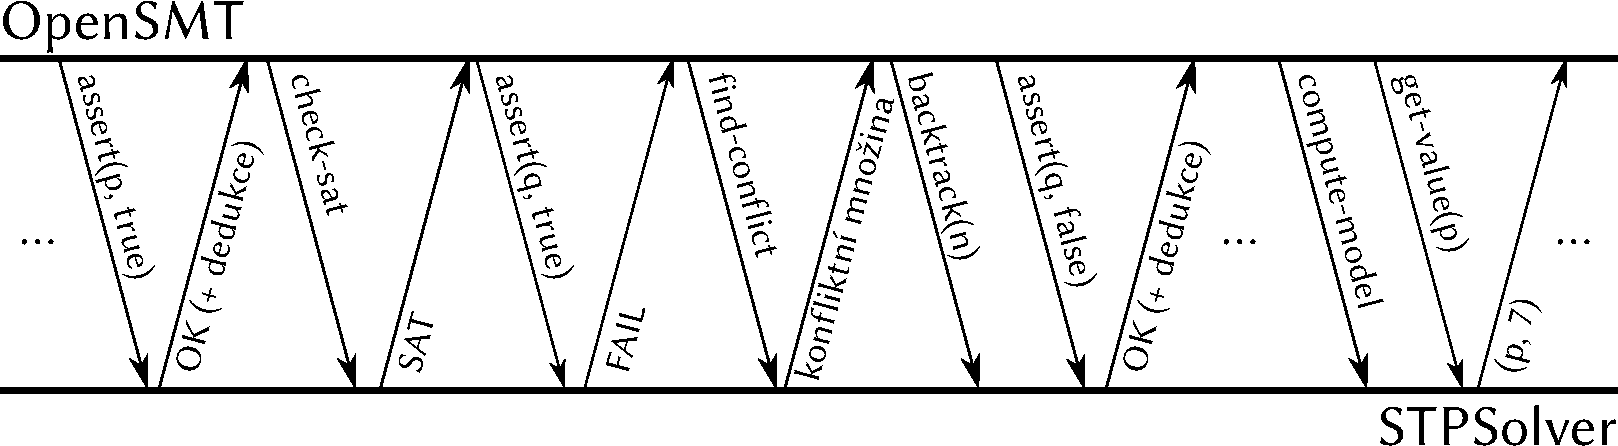
\includegraphics[width=\textwidth]{interface}
	\caption{Ukázka interakce řešiče s~OpenSMT (pseudokód)}
\end{figure}

V~první fázi algoritmu jsou řešiči předány všechny literály teorie, které se vyskytují ve vstupní formuli. Řešič z~nich nejprve extrahuje relevantní hodnoty. Následně zkontroluje, zda se nejedná o~negaci některého z~již zapamatovaných literálů. Pokud ano, pouze tuto negaci explicitně označí. V~opačném případě vytvoří hranu odpovídající tomuto literálu a~zároveň a~priori hranu tvořící negaci tohoto literálu, jak je popsáno v~sekci \ref{upravy}. Obě nové hrany se stanou součástí úložiště a~jsou zařazeny do překladových tabulek. Zbytek výpočtu pak již může předpokládat, že pracujeme pouze se známými literály, pro něž máme vytvořené hrany.

Poté, co jsou všechna omezení načtena, nastává hlavní část programu. Během té postupně řešič dostává rozhodnutá ohodnocení literálů. Když nějaké obdrží, přidá do omezujícího grafu hranu odpovídající tomuto ohodnocení. Následně proběhne prohledávání objevující všechny důsledky tohoto ohodnocení. Tyto důsledky jsou přeloženy zpět do vhodné formy a~oznámeny frameworku.

Po nějaké sekvenci těchto ohodnocení buď nalezneme splňující ohodnocení celé formule, nebo se dostaneme do sporu. Spor můžeme rozpoznat tak, že se chystáme přidat do grafu hranu, jejíž negace byla buď dříve do grafu přidána, nebo byla nalezena jako důsledek dřívějšího ohodnocení. V~takovém případě řešič oznámí selhání tohoto ohodnocení a~přejde do chybového stavu. Jakmile je řešič v~chybovém stavu, automaticky zamítá všechna nová ohodnocení. V~této situaci následuje nalezení nesplnitelné množiny. Pokud byla objevená negace hrany explicitně přidána do grafu, je tato množina triviální. Jinak ji získáme modifikovanou verzí prohledání grafu (viz.~\ref{alg}). Jakmile je nesplnitelná množina nalezena a~předána frameworku, rozhodne se podle ní úroveň backtrackingu. Ten je v~OpenSMT řešen obecně pomocí systému záchytných bodů. Řešič může být v~libovolnou chvíli požádán, aby uložil svůj aktuální stav na zásobník. V~případě nutnosti je mu pak sděleno, aby odebral několik bodů z~vrchu tohoto zásobníku a~tím se vrátil do dřívějšího stavu. 

Jakmile se řešič vrátí do konzistentního stavu, tento proces se opakuje, dokud není nalezeno nějaké splnitelné ohodnocení, nebo dokud framework nevyčerpá všechny možnosti ohodnocení. Splnitelnost formule je určena tím, který z~těchto dvou případů nastane. V~případě, že je formule splnitelná, může být řešič na závěr výpočtu ještě požádán, aby vytvořil její model, tedy nalezl konzistentní hodnoty pro všechny proměnné obsažené v~literálech teorie.

\section{Srovnání reálné a~celočíselné verze} \label{int_v_real}

Algoritmus uvedený v~sekci \ref{alg} je s~drobnými úpravami použitelný jak pro RDL, tak pro IDL. Přestože v~této práci implementujeme pouze celočíselnou verzi problému, přišlo nám názorné zamyslet se nad rozdíly mezi oběma variantami.

%Uveďme nejprve pro zajímavost, že pokud na vstupu podporujeme i~rovnice a~jejich negace, ověření konzistence je možné v~reálných číslech provést polynomiálně, zatímco pro celočíselný obor je ověření NP-těžké --- jsme schopni na něj převést např. problém $k$-barevnosti grafu \cite{slides}.

Prvním zjevným rozdílem pro potřeby naší implementace je reprezentace čísel. Reálná čísla je potřeba reprezentovat jinak, než čísla celá. OpenSMT definuje vlastní datový typ pro reálná čísla nazvaný \icode{FastRational}. V~různých částech kódu jej můžeme najít také pod aliasy \icode{Real} nebo \icode{Number}. Tento typ má několik výhod oproti běžným primitivním typům s~pohyblivou desetinnou čárkou. Především se jedná o~typ s~teoreticky neomezenou velikostí. Jelikož využívá struktur větších než jedno procesorové slovo, není limitován kapacitami procesoru. Důsledkem toho je to také typ s~libovolnou přesností. Netrpí tak zaokrouhlovacími chybami a~ztrátou platných číslic u~velkých hodnot jako např. \icode{float} a~\icode{double}. Tyto vlastnosti jsou důležité, jelikož sémantika SMT-LIB\footnote{sada standardů a~knihoven zabývající se SMT řešiči, vůči níž je OpenSMT implementováno} vyžaduje, aby všechny číselné výpočty probíhaly s~neomezenou přesností.

Samozřejmě bychom mohli \icode{FastRational} použít i~v~celočíselném řešení. Usnadnilo by nám to návrh datových struktur a~umožnilo větší znovupoužitelnost kódu. Testováním se však ukázalo, že aritmetické operace na \icode{FastRational} jsou citelně pomalejší než u~primitivních typů. Náš projekt tak používá primitivní celočíselný typ, konkrétně typ \icode{ptrdiff\_t}\footnote{\icode{ptrdiff\_t} byl vybrán jako znaménkový typ s~největším rozsahem, který můžeme na cílové architektuře očekávat}. Ten bohužel podporuje pouze hodnoty omezeného rozsahu a~je tak v~rozporu se standardem. Protože ale v~OpenSMT zatím neexistuje ekvivalent \icode{FastRational} pro celá čísla, uznali jsme jej jako nejlepší volbu. Toto rozhodnutí bylo podpořeno skutečností, že omezení rozsahu se experimentálně ukázalo jako zanedbatelné pro běžné použití --- z~661 testů knihovny SMT-LIB náš řešič vrátil ve všech případech správný výsledek (podrobněji viz.~kapitola \ref{experiment}).

Zásadní algoritmický rozdíl je také v~tvorbě negací. Máme-li například na vstupu nerovnici $(x-y<k)$, v~IDL ji triviálně převedeme do tvaru $(x-y\leq k-1)$. V~RDL se ovšem ostrých nerovností tak snadno nezbavíme. Nieuwenhuis a~Olivieras \cite{Nieuwenhuis05} navrhují pro tento případ postup, který využili např. Dutertre a~de Moura ve svém řešiči pro lineární aritmetiku \cite{Dutertre06}. Ten je založen na následujícím tvrzení.
\begin{tvrz}[Dutertre a~de Moura \cite{Dutertre06}, Lemma 1] 
	Nechť množina literálů lineární aritmetiky $\Gamma$ obsahuje ostré nerovnosti $S = \{p_1 > 0,\dots,p_n > 0\}$. $\Gamma$ je splnitelná právě tehdy, když existuje racionální $\delta > 0$ takové, že $\Gamma_\delta = (\Gamma \cup S_\delta) \setminus S$ je splnitelná, kde $S_\delta = \{p_1 \geq\delta,\dots,p_n \geq\delta\}$.
\end{tvrz}

Toto tvrzení umožňuje nahradit všechny ostré nerovnice neostrými, známe-li dostatečně malé $\delta$. Hodnotu $\delta$ přitom Dutertre a~de Moura nepočítají přímo, ale používají ho pouze symbolicky jako \emph{infinitesimální parametr}. Omezení a~proměnné pak nejsou ohodnoceny běžnými racionálními čísly, ale dvojicemi čísel $(c, k)$, reprezentujícími výraz $c + k\delta$, na kterých zavedeme odpovídající aritmetické a~porovnávací operace. Hodnotu $\delta$ je po této substituci třeba hledat až na samotném konci výpočtu, a~to pouze pokud potřebujeme najít model splňujícího ohodnocení. V~kontextu OpenSMT už je tento přístup použit rovněž v~řešiči teorie lineární aritmetiky.

